%!TEX root = ../../PhD_thesis__Edouard_Leurent

\graphicspath{{2-Chapters/1-Chapter/}}

\chapter{Introduction}
\label{chapter:1}

\begin{flushright}
	\begin{tabular}{@{}l@{}}
		\emph{Pour soulever un poids si lourd,}\\
		\emph{Sisyphe, il faudrait ton courage !}\\
		\emph{Bien qu’on ait du cœur à l’ouvrage,}\\
		\emph{L’Art est long et le Temps est court.}\\
	\end{tabular}
	
	Charles Baudelaire, \href{https://eleurent.github.io/sisyphe/texts/le-guignon.html}{\emph{Le guignon}}.
\end{flushright}

\section{Context and scope}

% Moral Machine
% Not implement solutions to moral dilemmas, but consider the non-dilemma of avoiding accidents

\begin{figure}[tp]
	\centering
	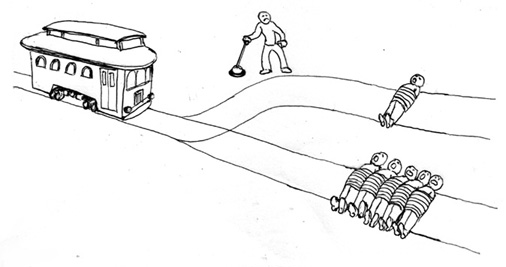
\includegraphics[trim={0 5cm 0 5cm}, clip, width=0.7\linewidth]{img/trolley}
	\caption{The Trolley problem variant considered in this work. Design by \href{https://www.teepublic.com/fr/pin/685858-there-is-no-problem.-you-are-travelling-safely-to-}{penguino}.}
\end{figure}

\section{Our contributions}
\section{Outline}
\section{List of publications}